%%%% 
% This is a template for project reports in the subject DAT620 at the
% Department of Electrical Engineering and Computer Science,
% University of Stavanger.
% 
% The template is based on the ACM conference template 
% it was edited by Leander Jehl and Hein Meling
\documentclass[sigconf]{acmart}

%DON'T CHANGE THIS FILE
%This file sets several properties for the ACM template.
%It is not necessary to change this file.


% Copyright
\setcopyright{none}

% DOI
\acmDOI{}

% ISBN
\acmISBN{}

%Conference
\acmConference[Project in Computer Science (DAT500)]{}{IDE}{UiS}
\acmBooktitle{}
\copyrightyear{2020}

\newcommand{\supervisors}[1]{\thanks{Supervised by #1}}

%In the preamble file you can include packages and define macros.
\usepackage{xspace}

%Here we define a marco: The \xspace ensures correct spacing, i.e. insert space before next word, but not before period or comma.
\newcommand{\paxos}{\textsc{Paxos}\xspace}
\newcommand{\csv}{\textsc{csv}\xspace}

\usepackage[utf8]{inputenc}
\usepackage[english]{babel}
\usepackage{fancyhdr}
\usepackage{lastpage}
\usepackage{tikz}
\usepackage{pgfplots}
\pgfplotsset{compat=newest}




\pagestyle{fancy}
\fancyhf{}

\rfoot{Page \thepage \hspace{1pt} of \pageref{LastPage}}



\begin{document}
\title{Crypto market analysis prediction in distributed systems}
\subtitle{DAT500 - Final Project Report}

\author{Asahi Cantu Moreno}
\affiliation{University of Stavanger, Norway}
\email{a.cantumoreno@stud.uis.no}

\author{Daniel Urdal}
\affiliation{University of Stavanger, Norway}
\email{d.urdal@stud.uis.no}

\supervisors{Jayachander Surbiryala, Tomasz Wiktorski
Tomasz Wiktorski,Markus Pettersen
Markus Pettersen}



\begin{abstract}
The creation of cryptocurrency and its exponential adoption over the last three years  has led to the creation of many different exchange and tools to trade it via Internet. Unlike common stock trading, cryptocurrency works nonstop all year with simple and advanced interfaces, allowing anyone with a minimum investment to enter the market and exchange assets in real time, with high liquidity and asset availability. Because of the early state of the technology and the socioeconomic-political factors affecting the regulation of the cryptocurrency markets as well as the speed at which transactions are made has led to a high risk-high volatility market, making very hard to analyze or predict prices that can lead to profits for a chosen currency. This academic report contains a deep analysis on crypto market and aims to generate a prediction model by analyzing historical data, the news and events that can potentially affect the market and its impact on the prices by using distributed systems Hadoop® and Apache Spark® for data storage and interaction. Machine Learning models are implemented as well for a big data set. Further analysis, results and potential for future work is presented in this report.
\end{abstract}

\keywords{Cryptocurrency, Machine Learning, Hadoop, Spark, Neural Networks, Distributed Systems}

\maketitle

\section{Introduction}
\label{sec:introduction}

\noindent
It was not long ago that bitcoin and the concept of Blockchain appeared for the first time on the Web as a white paper, October 31st 2008 to be more precise “Bitcoin: A Peer-to-Peer Electronic Cash System” \cite{nakamoto_bitcoin_2008} Said the document in its heading. It was uncertain by that time how disruptive such technology could be, and the importance of its role nowadays. A decade later, Bitcoin has consolidated as a strong and reliable asset in which people trust to invest and transfer money. The term “Cryptocurrency” was born. Little after its emission and open source code publication, several teams and individuals started re adapting its code and creating different electronic assets, slowly with its adoption a philosophy more people started trading on their private markets. It would not take too long to foresee the creation of a community and a market craving to trade different assets. As a result of this crescent demand Cryptocurrency market exchanges were created. From the financial perspective, cryptocurrency markets are nowadays allowing people who did not have access to credits or bank accounts before to enter into a different economic world were markets do not sleep, moreover assets can be instantly traded, changed and transferred. Years ago, this market consolidated and matured, data is produced massively, regulations or innovations, even political situations have made the market very peculiar and volatile, something unprecedented in the financial trading.

\begin{figure}[ht]
   \centering
   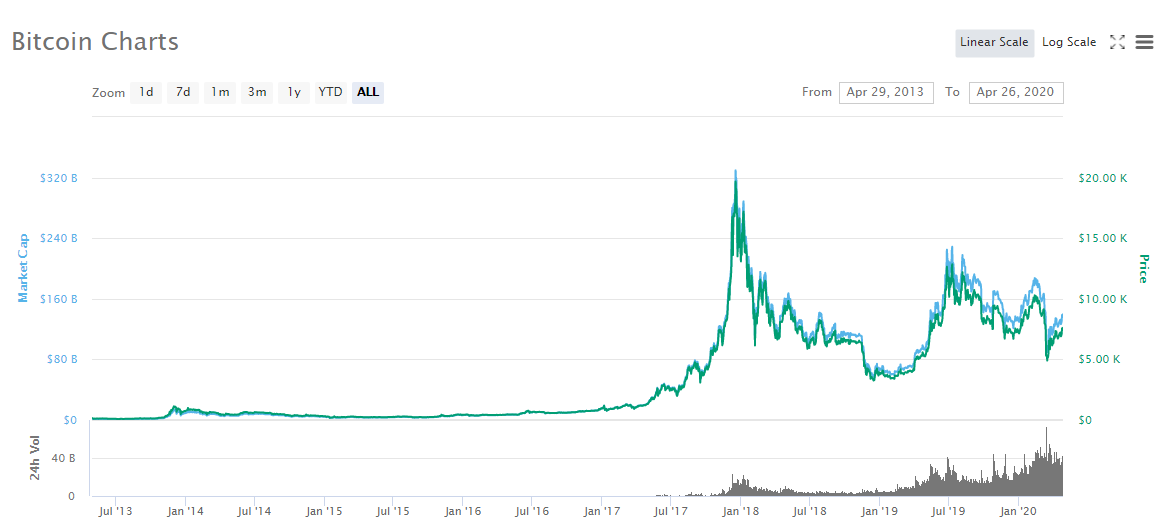
\includegraphics[width=\linewidth]{fig/BitcoinPriceChart.png}
    \caption{Bitcoin price chart (taken from \cite{coinmarketcap_bitcoin_2020})}
    \label{fig:BitcoinChart}
\end{figure}

Bitcoin price volatility generated a high-risk market, but also a lot of interest and market capitalization has been set to the cryptocurrency assets. On April 2020, the total market capitalization of all cryptocurrencies is up to  \$219,165,492,833.00 USD \cite{coinmarketcap_cryptocurrency_2020} which translates in a growing market accessible to anyone with sufficient resources around the world to trade. As the time goes by more resources and assets will be added resulting in an expected increase of profit depending on the investment, but daily fluctuations are visible as well for any asset.

In addition to this, the impact of social media and published news about recent technological progress and Information Technology improvements are expected to be a key player in the decision different traders made to trade cryptocurrency assets. There might be a direct correlation in what is published on social media, news and the price fluctuation of the market in short term basis. It is therefore the aim of this report to explore, discover and predict potential market prices through distributed systems to show the potential of creating a scalable product trained to predict short term prices according to past fluctuations and media publications. 
The system used, algorithms, data set and brief explanation of the challenges in addition to obtain results will be explained in detail though this report. Provided results can be also used as a basis for future work development and algorithm improvements.

\section{Background}
\label{sec:background}
The growing importance of cryptocurrency in a global market where facing a potential economic crisis in which fiat money might not be anymore the common exchange medium between different parties. The technological development and amazing availability of growing data to explore are the key factors that led to research on cryptocurrency and try to analyze through machine learning and distributed systems the potential price fluctuations. 
Another point to consider: Social media plays nowadays an important role in our daily life, more and more politicians use these platforms for instant communications, researchers announce publications and press uses them as a main platform to publish breaking news. All in all, we cannot take out anymore social media from the impact of our economic and political situations. It is therefore important to consider this as a key factor in the market decisions made on daily basis and the price fluctuations of the assets.

The main idea is to use a big cryptocurrency data set and a trained model of cryptocurrency related news to predict short term future prices for all the provided asset by using Machine learning algorithms. 

\subsection{Cryptocurrency}

Cryptocurrency can be defined as “a digital asset designed to work as a medium of exchange that uses strong cryptography to secure financial transactions, control the creation of additional units, and verify the transfer of assets.” \cite{noauthor_what_2020} Cryptocurrencies use decentralized control as opposed to centralized digital currency and central banking systems, which means no central entity has full control or power over the asset, but the community maintains it through systems known as “nodes” and each transaction is recorded in a public ledger known as the “blockchain”\footnote{A blockchain is a time-stamped series of immutable records of data that is managed by a cluster of computers not owned by any single entity. Each of these blocks of data (i.e. block) is secured and bound to each other using cryptographic principles (i.e. chain). public to anyone and resilient to changes. It is therefore virtually impossible to commit fraud if more than 50\% of the computational resources belong to the community and not the entity intending to hack or modify the blockchain\cite{ameer_rosic_what_2016}}

\subsubsection{Cryptocurrency Data set}

The data set used for this project is a Binance exchange data set extracted from the portal Kaggle\cite{smit_binance_2020}. The data set is titled “Binance Full History” and contains 1 minute candlestick data for a total of 786 cryptocurrency pairs traded on the exchange Web portal Binance.com\cite{binance_bitcoin_2020}. 
The features of this data set are:
\begin{itemize}
    \item Data types: python-pandas parquet files\footnote{pandas is a Python package providing fast, flexible, and expressive data structures designed to make working with "relational" or "labeled" data both easy and intuitive. It aims to be the fundamental high-level building block for doing practical, real world data analysis in Python \cite{noauthor_pandas_2020}. Parquet files are compressed binary files specially built to reduce storage size of big data files and improve loading performance.}
    \item Data size : 10GB
    \item Number of files : 764
\end{itemize}

\begin{figure}[H]
   \centering
   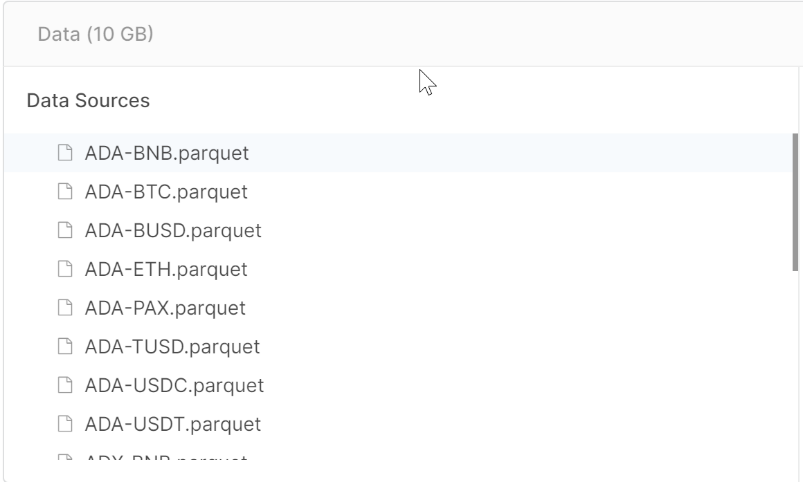
\includegraphics[width=\linewidth]{fig/CryptocurrencyDataSetParquetFiles.png}
    \caption{Cryptocurrency data set. Parquet file (taken from \cite{smit_binance_2020})}
    \label{fig:CryptoCurrencyDatasetParquet}
\end{figure}

\subsubsection{Cryptocurrency data set features and details}

A minute candlestick represents the maximum and minimum price at which any given asset was sold. It also contains information about the open price (price at the beginning of the time) and close price (end of time). 

\begin{figure}[h]
   \centering
   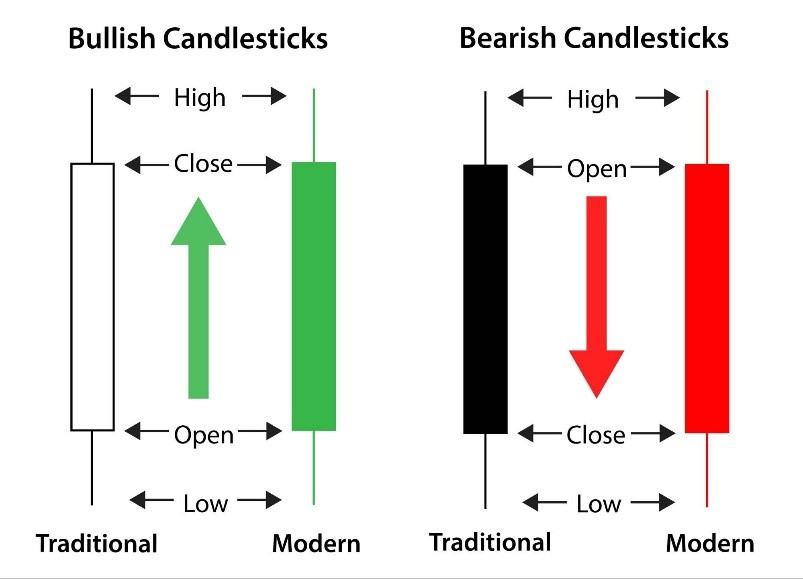
\includegraphics[width=\linewidth]{fig/CandlestickRepresentation.jpg}
    \caption{Candlestick Representations}
    \label{fig:CryptoCurrencyDatasetParquet}
\end{figure}

A series of candlestick represent the market fluctuation in a given period of time. 

\subsection{News data set}

The news data set was extracted from the web portal “CoinTelegraph.com”\footnote{The most recent news about crypto industry at Cointelegraph. Latest news about bitcoin, ethereum, blockchain, mining, cryptocurrency prices and more\cite{cointelegraph_cointelegraph_2013}} .
The data set was created using python scripts due to the lack of availability of a full set. 

The features of this data set are:

\begin{itemize}
    \item Data types: 2 \csv files total size is 128 MB.
    \item More than 20,000 different news from 2013 until present for human-written news about cryptocurrency and related subjects.
    \item Header file. Contains relevant metadata information about the news (such as title, thumbnail, creation date, etc.).
    \item Content file. Contains the body of the news and other metadata like the number of views and times it has been shared as well as image references for it.
\end{itemize}

\begin{figure}[h]
   \centering
   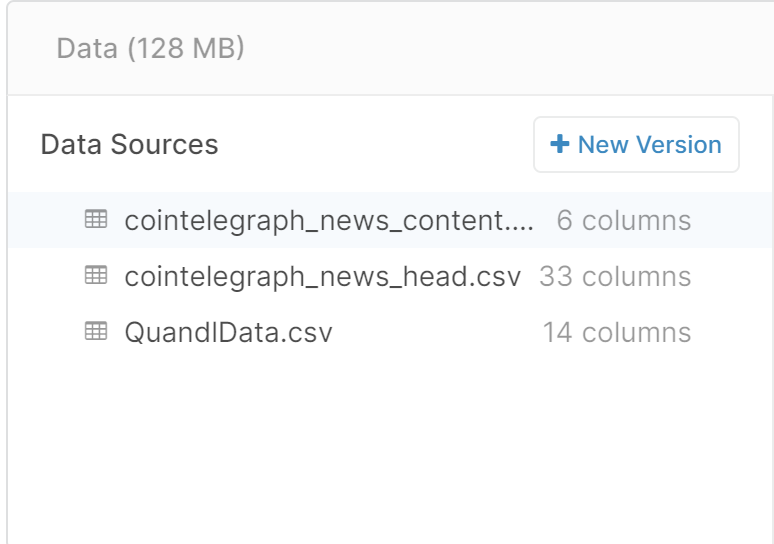
\includegraphics[width=\linewidth]{fig/CryptocurrencyNewsDataSet.png}
    \caption{Cryptocurrency News Data set \cite{cantu_cryptocurency_2020}}
    \label{fig:CryptoCurrencyNewsDataset}
\end{figure}


\subsection{Related works}
Several attempts and previous works from the data science community have been made to predict stock market price using Machine learning. The procedures and models are not so much different from the cryptocurrency model since both are time series models and its current input depend directly on past data. There is, however one big difference: the price volatility, which leads to the research no model training and adjustment to compensate for the possible increases and at the same time adapt the model to avoid overfitting.

For this project and among other sources three jobs were considered as role models:

\citeauthor{xavier_predicting_2019} approaches in his research document different Machine Learning models and mechanisms to predict tock market prices by performing Moving Average and LSTM\footnote{Acronymm for Long Short-Term Neural network. A special kind of Neuran network model that is trained based on past data.} training models. His results show the differences in the accuracy for the two different models and make evident that LSTM model performs better, although several adjustments have to be done depending on the asset to model.  \cite{adusumilli_predicting_2020} 

\citeauthor{pablo_castilla_predict_2018} takes the theory of LSTM into practice in a kaggle document, and figures the basic mecanishm for data processing, normalization and training\cite{pablo_castilla_predict_2018}.

Finally the work from \citeauthor{sagar_cryptocurrency_2019} addresses the machine learning mechanisms for cryptocurrency trading. Part of his research is used to tune and develop the Machine learning algorithms.







\section{Environment Setup}
\label{sec:method}
The system used for this for this project consisted of four virtual machines (VMs) running Ubuntu Server 16.04. Apache Hadoop version 3.2.1 was installed on each machine, and they were configured to run as a Hadoop cluster using the YARN resource manager. They were configured such that one VM acted as a master node, while the other three acted as slave nodes.
Apache Spark was installed using the 3.0.0 preview version, as this was the only version supporting Hadoop 3.2.1. In order to get Spark running on the VMs, Python version 3.8.1 was compiled from source and installed alongside the default Python 2.7.12.

\section{Data processing}
\label{sec:method}
The goal is to combine both data sets, transform them when necessary to reduce size, features and use them with ML training algorithms that enable an accurate cryptocurrency market price prediction.

\subsection{Cryptocurrency data set processing}

Because this data set was machine-generated little had to be done to process it. It was important, however, to examine the contained information and extract just the necessary one in real time. Because of data size, and the technical resources limitations it was not possible to extract and store the required information, but rather open the file, select the main features and use them in real time for machine learning algorithm to train and generate a model, and the close it. Uncompressed data reached 70 GB of space, whereas compressed data set just 9 GB.

\subsubsection{Data set description and feature selection}
Each parquet file in the data set contains the corresponding information as shown in Figure 5. 


\begin{figure}[H]
   \centering
   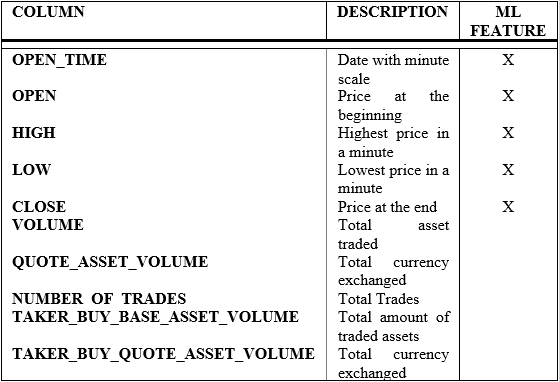
\includegraphics[width=\linewidth]{fig/Cryptocurrency features.png}
    \caption{Cryptocurrency features}
    \label{fig:CryptocurrencyFeatures}
\end{figure}

\begin{figure}[H]
   \centering
   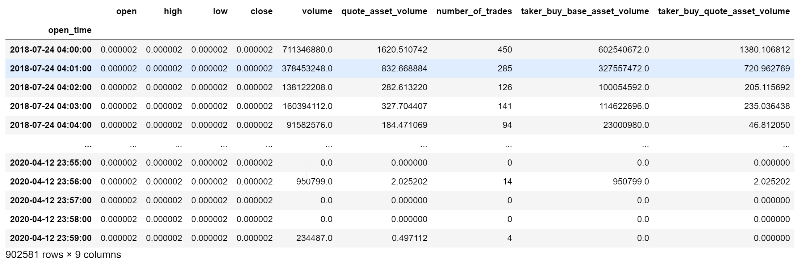
\includegraphics[width=\linewidth]{fig/ExampleParquetFile HOT-ETH.png}
    \caption{Example of parquet file HOT-ETH.parquet}
    \label{fig:CryptocurrencyDataSetParquetFile}
\end{figure}

From \ref{fig:CryptocurrencyFeatures} features marked with ‘X’ where selected to be processed and to train the Machine Learning model.

\subsection{Cryptocurrency news data processing}
This data set was non-existent, it had to be generated by creating a python script to bring the information from the web portal “coinmarketcap.com”. The script uses web scraping methodology and extracts the news set according to the given parameters.  
A total of 24519 news articles had to be gathered and processed to generate the data set in two steps.
The first step consists on getting the header information from the web portal, whereas the second brings the content of a specific  news article.
 The script was generated and run in a Hadoop cluster to better control and preserve information in case of data loss. 
A part of the algorithm is shown, full code description and implementation can be seen in \cite{christopher_olah_understanding_2015}.

\begin{figure}[H]
   \centering
   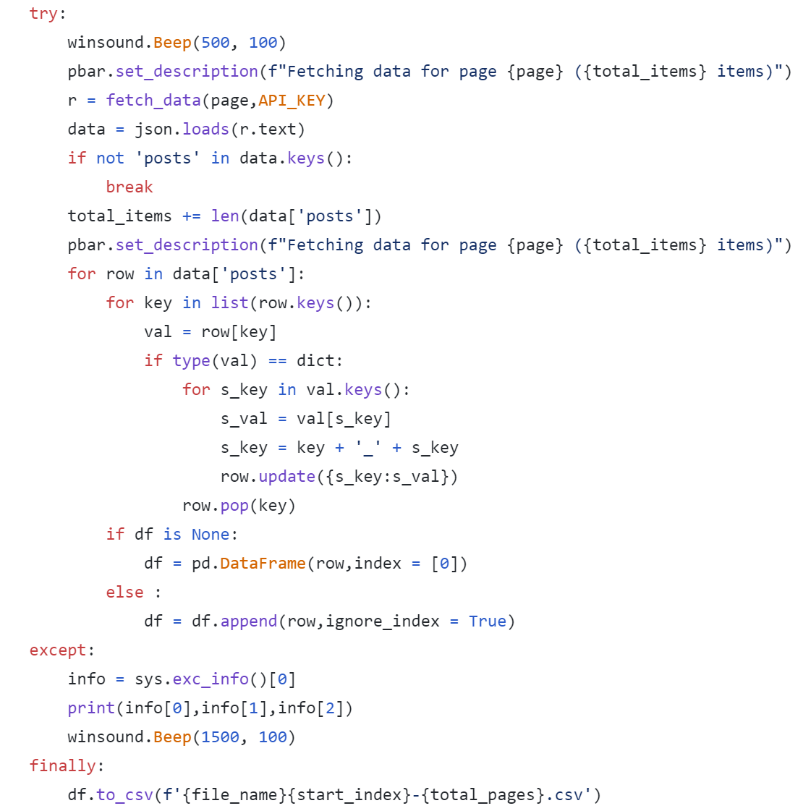
\includegraphics[width=\linewidth]{fig/CodeSnippetNewsHeading.png}
    \caption{Code implementation for news heading extraction. Data is extracted into a dictionary and later saved on a pandas DataFrame}
    \label{fig:CodeSnippetNewsHeading}
\end{figure}

\begin{figure}[H]
   \centering
   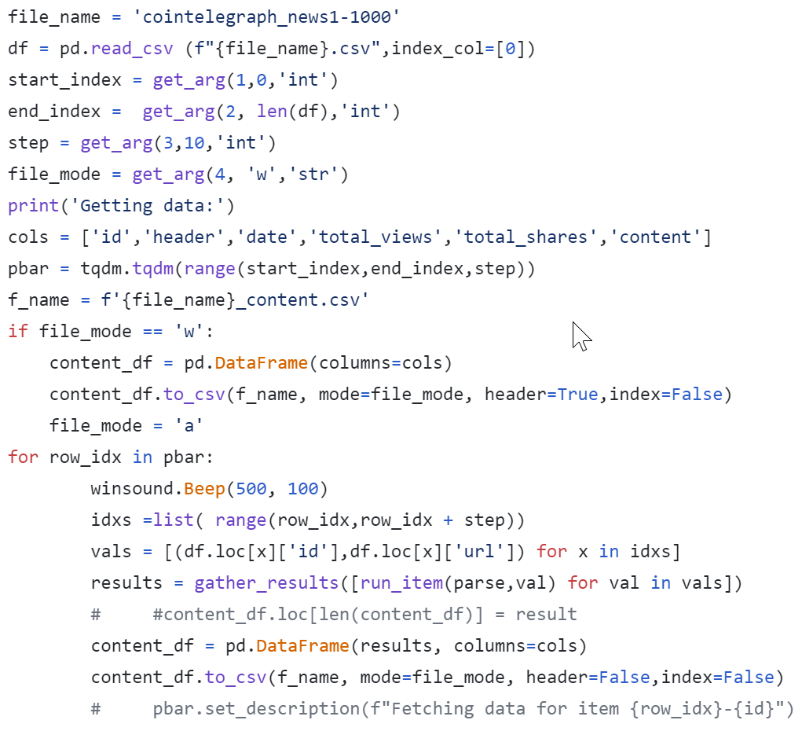
\includegraphics[width=\linewidth]{fig/CodeSnippetNewsContent.png}
    \caption{Code implementation for news article extraction, data is directly saved in a pandas DataFrame and updated in a csv file. http request interactions are intensive and took close to 3 days of continuous execution to retrieve the full data set}
    \label{fig:CodeSnippetNewsContent}
\end{figure}

Once created the data set, it was properly cleaned and processed to be used for natural language processing just one file (cointelegraph\textunderscore news\textunderscore content.csv) was used to train the model for being the one with the article content.

\begin{figure}[H]
   \centering
   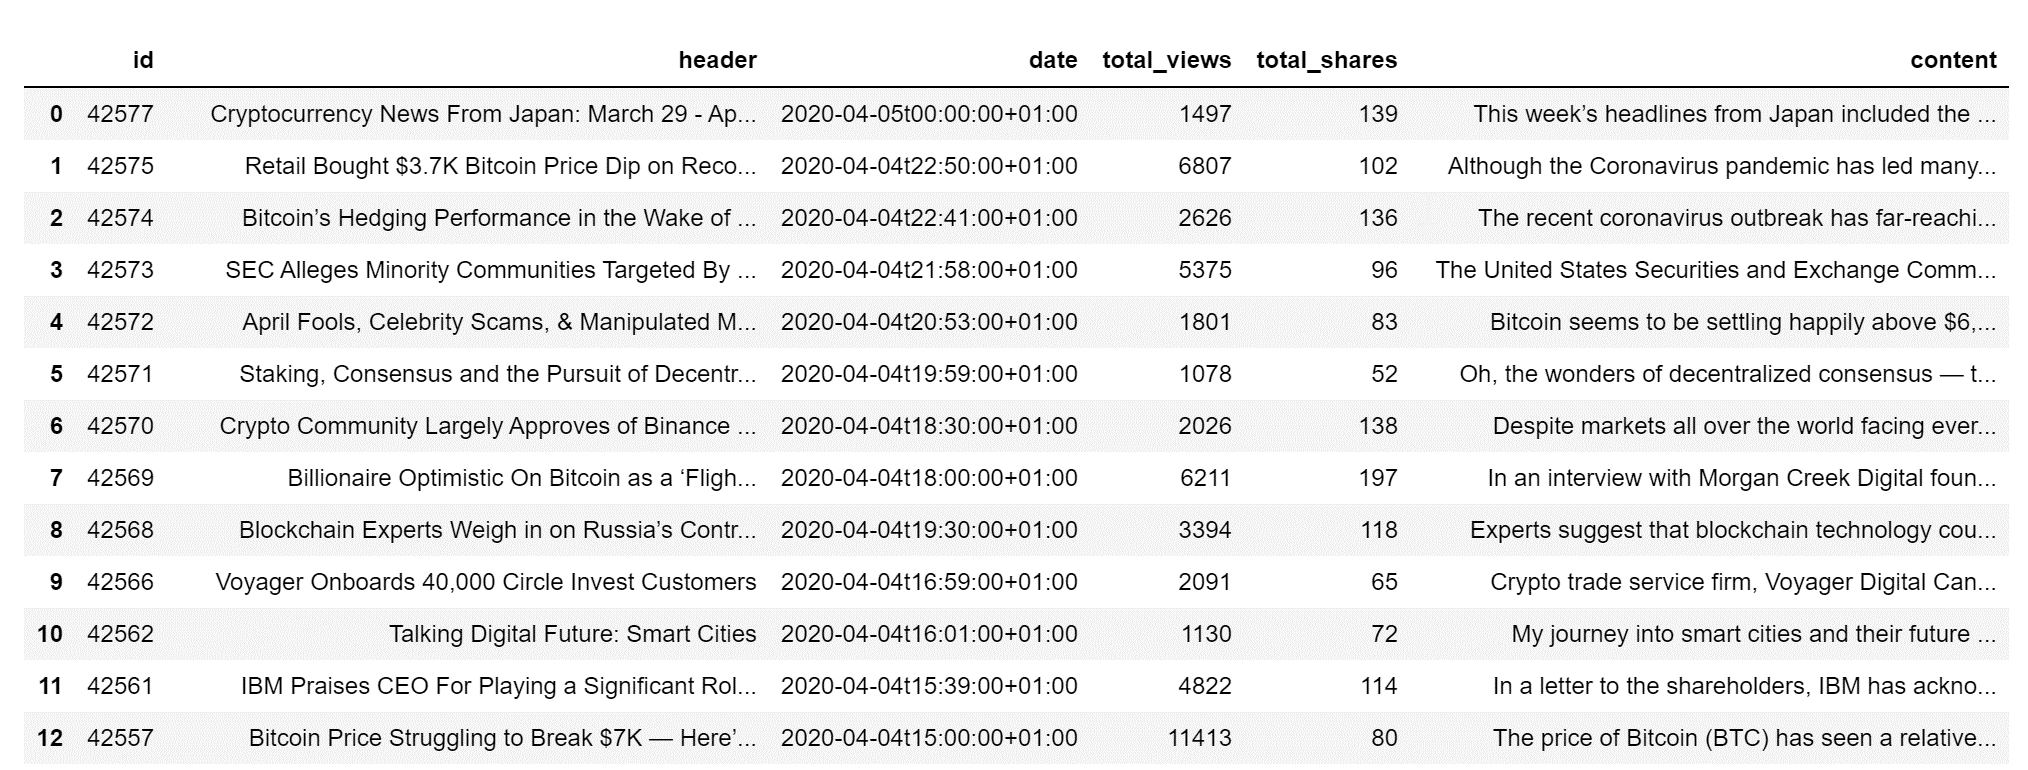
\includegraphics[width=\linewidth]{fig/NewsContentExample.png}
    \caption{Cryptocurrency news content example}
    \label{fig:NewsContentExample}
\end{figure}


\section{Algorithm implementations}
\label{sec:method}
Unlike other Machine Learning algorithm applications to systems  and problem, stock trading belongs to a particular branch of algorithm implementation: sequence prediction problems, which tend to prediction of current and next values depends on the history and past records, events do not occur independently. For these situations RNN\footnote{Recurrent Neural Networks, is a class of artificial neural networks where connections between nodes form a directed graph along a temporal sequence\cite{christopher_olah_understanding_2015}}  algorithms are applied to the cryptocurrency candlestick data set\cite{mittal_understanding_2019}.

On the other hand, for the news feed data set it was decided to implement NLP\footnote{Natural Language Processing} algorithms and clustering for unclassified text, since the data set is not labeled. The intention of such classification was to better understand the topics for the news, to isolate, classify them and try to find a pattern to categorize the news. Subsequently a sentiment analysis algorithm can be performed to generate a label that determines whether a specific article is positive or negative, and how meaningful it is for the trading in during the next hours or days. The assumption is that by this results forecasts can be more accurate as they can take articles in real time and merge them with the candlestick data to adapt the training model into a more realistic prediction.

\begin{figure}[H]
   \centering
   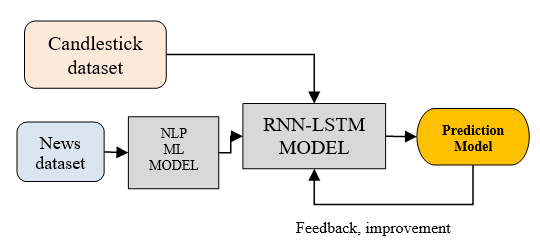
\includegraphics[width=\linewidth]{fig/RNNLSTM.png}
    \caption{ML Training model prototype}
    \label{fig:RNNLSTM}
\end{figure}

\subsection{Cryptocurrency analysis algorithm}

Memory-based networks such as Recurrent Neural Networks (RNN) and Long Short-Term Memory (LSTM) networks allow for predictions to be remembered and forgotten; this can be useful when predicting extreme changes in a short space of time via the remembering of previous examples. Compared to other models, RNN and LSTM are suited towards sequential data such as stock prices, whereas other models must take a non-sequential, sample-independent interpretation of the data, considering only a single input and output sample at a time \cite{chen_lstm-based_2015}

\begin{figure}[H]
   \centering
   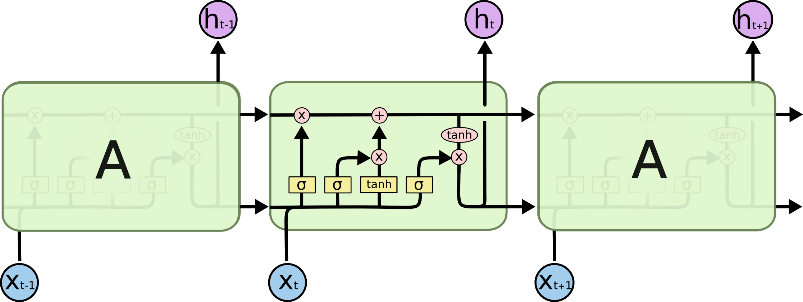
\includegraphics[width=\linewidth]{fig/RNNLSTM2.png}
    \caption{Example of a RNN-LSTM model}
    \label{fig:RNNLSTM2}
\end{figure}

To implement RNN-LSTM approach the python TensorFlow\footnote{TensorFlow is a free and open-source software library for dataflow and differentiable programming across a range of tasks. It is a symbolic math library, and is also used for machine learning applications such as neural networks. Package can be downloaded from \hyperref[https://www.tensorflow.org]{https://www.tensorflow.org}}  deep learning model package was used and adjusted for the best-case scenario in which the loss function and consequent prediction were as accurate as possible without much overfitting. Several examples were observed, the model was retrained for all the cryptocurrency assets using spark functionality with Hadoop ass a file system \cite{yacoub_ahmed_predicting_2019}. 

\subsection{Text and technical sentiment analysis algorithm}

News data set was intended to be classified and processed by using Natural Language processing tools and algorithms to find patterns in the whole dataset. Normal processes for NLP processing require (among others):
\begin{itemize}
    \item String tokenization
    \item Stop words removal
    \item Lexicon normalization
    \item Lemmatization method was applied
    \item Word2Vet approach implemented as well
\end{itemize}

Several NLP and sentiment analysis algorithms were used to classify the model and try obtaining the news topics:

\begin{itemize}
    \item K-Means Clustering
    \item Treating with an unlabeled data set for cryptocurrency news required a machine learning model to try to process and generate corresponding clusters in order to identify the main topics
    \item Sentiment analysis
    \item Common sentiment analysis was performed over the full dataset. This approach aimed to find and tag an approximate positive, neutral or negative sentiment to each document.
    \item Pre-Trained data models
    \item The existence of complex machine learning models based on big scientific documents were used to try to identify and label each article
    \item Text summarization
    \item Extractive summarization approach was performed to try to identify the main topics

\end{itemize}



\section{Code implementations}
\label{sec:method}
The majority of the algorithms were implemented thinking on a distributed system approach in which data intensive processes and redundancy systems could be able to handle the provided information. The configuration employed is listed below:

\begin{itemize}
    \item Hadoop Cluster (Ubuntu System)
    \item 1 Name Node (Master)
    \item 3 Data Nodes (Slaves)
    \item Apache Spark as the processing interface with PySpark
    \item Spark Dataframes
    \item RDD’s and distributed processes
    \item Jupyter notebook for python scripting
    \item Tensorflow as the machine learning package
    \item Intended to use SparkML
    \item NLP Packages and tools:
    \item NLTK
    \item Spacy
    \item VaderSentiment
    \item Textblob
    \item Textacy
    \item Gensim
\end{itemize}

\begin{figure}[H]
   \centering
   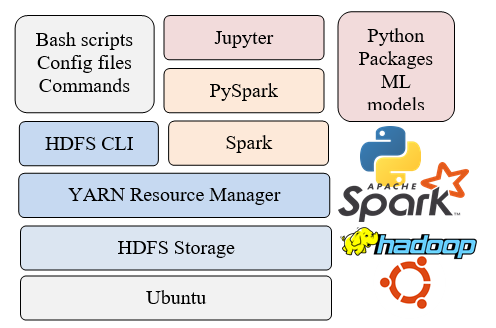
\includegraphics[width=\linewidth]{fig/serverarchitecture.png}
    \caption{Distributed system architecture}
    \label{fig:serverarchitecture}
\end{figure}

\subsection{Cryptocurrency dataset code implementation}

The code for the cryptocurrency candlestick dataset was divided in three different python files

\begin{itemize}
    \item Settings file \textbf{crypto\textunderscore params.py}
    \begin{itemize}
        \item Contains a predefined set of variables, resulted from the training and tuning of the RNN-LSTM model. The most optimistic approach ad loss function implemented can be visualized here
    \end{itemize}
    \item ML algorithm  \textbf{crypto\textunderscore utils.py}
    \begin{itemize}
        \item Contains a code snippet for the ML training model and the configuration of its layers. The way it is called and used by TensorFlow
    \end{itemize}
    \item Data set reading and training in Spark  \textbf{sprk.ipynb}
    \begin{itemize}
        \item Is a Jupyter notebook that contains the main functionality and coordination to call the settings and utils files, respectively. In addition it sets the environment to open a spark environment and connect to the Hadoop YARN resource manager, which allows the system to read the parquet files in a distributed manner.
        \item Once the files are called, the ML model is called to be trained based on the obtained data set and the result is saved in a spark json format. This allows spark to save back the trained model in the distributed system, eventually as the data keeps growing the model will be  fed in an iterative process to readjust the prediction
    \end{itemize}
\end{itemize}

\begin{figure}[H]
   \centering
   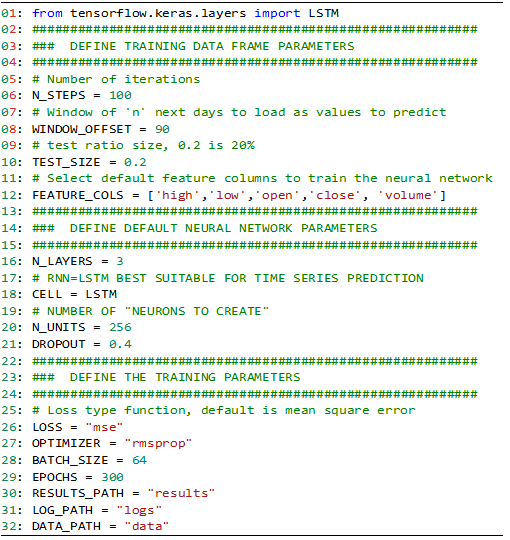
\includegraphics[width=\linewidth]{fig/CodeSnippetMLSettings.png}
    \caption{Fragment from file  crypto\textunderscore params.py}
    \label{fig:CodeSnippetMLSettings}
\end{figure}

\begin{figure}[H]
   \centering
   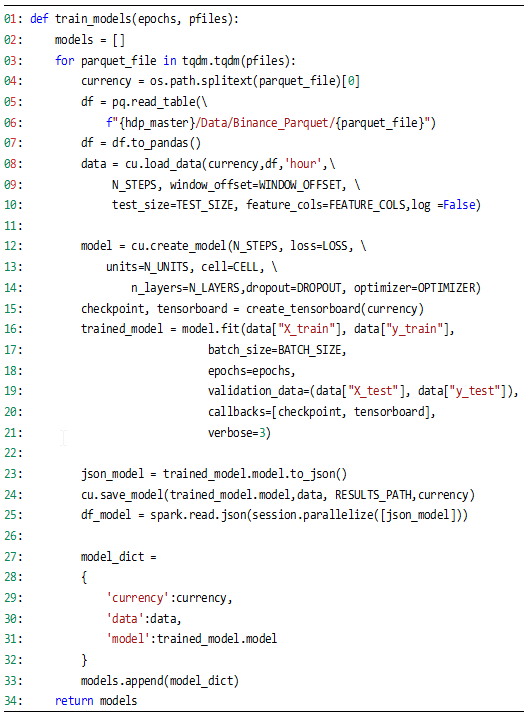
\includegraphics[width=\linewidth]{fig/CodeSnippetMLMain.png}
    \caption{Fragment from file  crypto\textunderscore utils.py}
    \label{fig:CodeSnippetMLTraining}
\end{figure}

\begin{figure}[H]
   \centering
   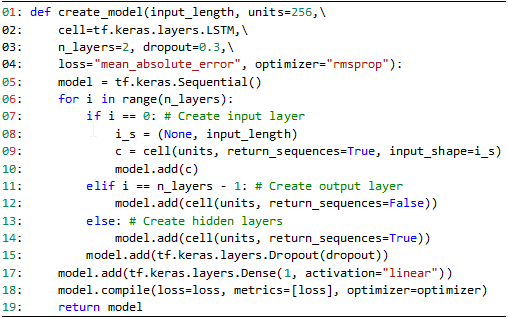
\includegraphics[width=\linewidth]{fig/CodeSnippetMLTraining.png}
    \caption{Fragment from file  crypto\textunderscore sprk.ipynb}
    \label{fig:CodeSnippetMLMain}
\end{figure}

\section{Newsfeed data set code implementation}
The newsfeed data set code required a special treatment. It consisted of two stages:

\subsubsection{Stage 1. Newsfeed data set extraction}

Since the whole data was not available on the web, a python script had to be developed in order to store such the information from the known sources. The implementation of such script is very important due to the lack of the information on the web. The script sets the basis for anyone else to use it and implement the code for any other newsfeed to assemble different data repositories. Both data set and code implementation have been published and made open for anyone to use it and improve it if required. The algorithm was developed in two scripts:
\begin{itemize}
    \item Newsfeed headings extraction
    \item Newsfeed articles extraction
\end{itemize}

\begin{figure}[H]
   \centering
   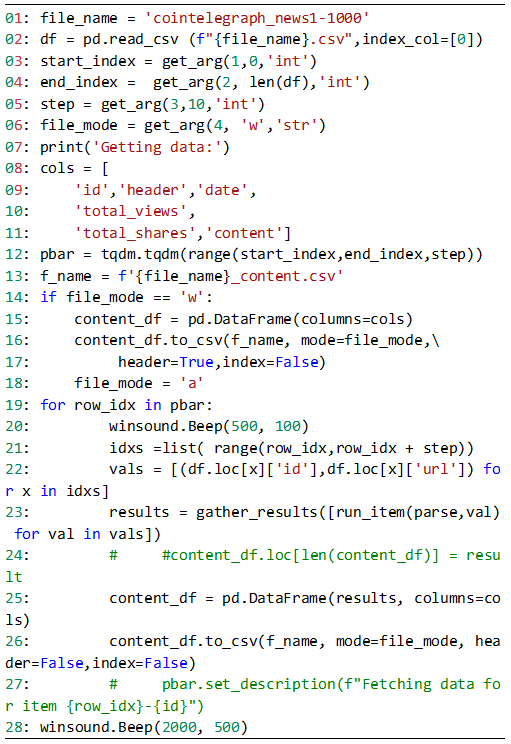
\includegraphics[width=\linewidth]{fig/CodeSnippetNewsHeadingExtraction.png}
    \caption{Code snipped for news headings extraction}
    \label{fig:CodeSnippetNewsHeading}
\end{figure}

\begin{figure}[H]
   \centering
   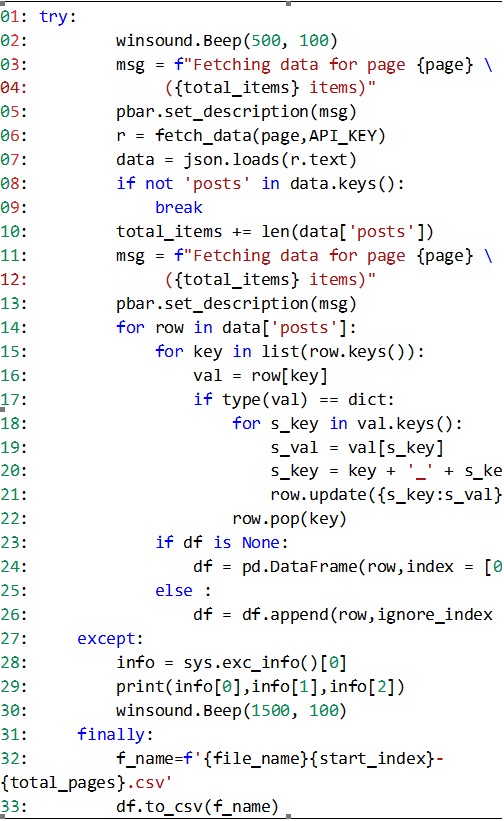
\includegraphics[width=\linewidth]{fig/CodeSnippetNewsContentExtraction.png}
    \caption{Code snipped for news articles extraction}
    \label{fig:CodeSnippetNewsContent}
\end{figure}

\subsubsection{Stage 2. Newsfeed exploration and classification}

Several attempts to classify the data set and train it to obtain relevant information that lead to decide whether an article is positive, or negative were performed. As stated in section 5.2, different approaches and analysis were tried to obtain a proper classification. Sentiment analysis, clustering, text summarization and deep learning algorithms were applied to the data set, the classification results were neutral and did not provide insightful information for the whole data set to be used and applied as an extra feature for the candlestick data set in the RNN-LTSM algorithm.

The code snippets shown below will demonstrate the use of such algorithms and the way to try to obtain useful information to tag the data set. It was observed, however, that such attempts were not enough and further text analysis was required. This is a limitation will be addressed in the next section.

\begin{figure}[H]
   \centering
   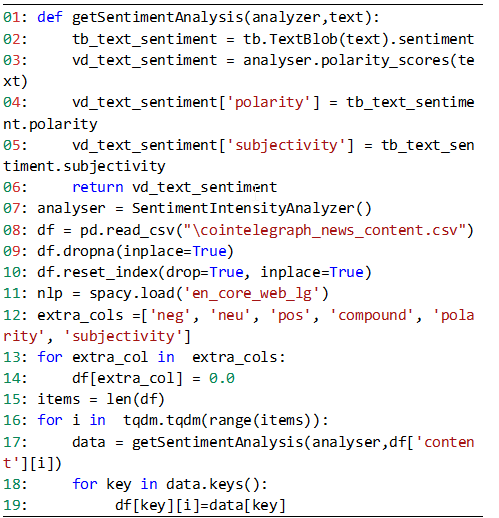
\includegraphics[width=\linewidth]{fig/CodeSnippetSentimentAnalysis.png}
    \caption{. Code snippet for sentiment analysis attempt}
    \label{fig:CodeSnippetSentimentAnalysis}
\end{figure}

\begin{figure}[t]
   \centering
   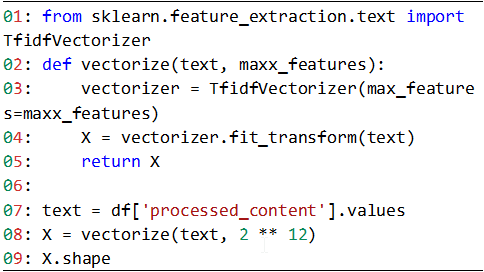
\includegraphics[width=\linewidth]{fig/CodeSnippetVectorization.png}
    \caption{Code snippet for text vectorization}
    \label{fig:CodeSnippetVectorization}
\end{figure}

\begin{figure}[H]
   \centering
   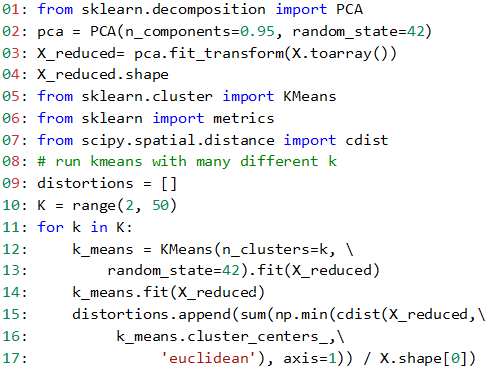
\includegraphics[width=\linewidth]{fig/CodeSnippetSentimentProcess.png}
    \caption{Code snippet for KNN clustering classification}
    \label{fig:CodeSnippetSentimentProcess}
\end{figure}




\section{Model training and tuning}
\label{sec:method}
Several iterations were required to get proper adjustments to the LSTM model for candlestick data and KNN for the NLP processing. The iterations involved observing the loss function through the deep learning model using TensorBoard and analyzing its precision, overfitting and underfitting on both models.

\subsection{Cryptocurrency data set training and tuning }

The final adjustments for the training of the neural network can be seen in [12]. The neural network implementation, training and performance for every cryptocurrency trained on the spark environment can be visualized as well in the provided citation. Each candlestick data set is processed in a pandas DataFrame. The loss function and window offset (period in which the neural network predicts the values based on past data) were carefully chosen to approximate the prediction as much as possible for all the sets. Primarily, it was observed that on average most of the models adapt properly at 300 epochs\footnote{The number of epochs is a hyperparameter that defines the number times that the learning algorithm will work through the entire training data set\cite{brownlee_when_2018}}  with “Mean Square Error” as loss function and 256 neurons on 3 layers (one hidden). The model can mutate, and it is let to the reader to try to find a better tuning mechanism. It is important to highlight that for the given model the data set was aggregated to present hourly data instead of minute. The reason for this was for the expensive of the process and the amount of resources a training model takes for a single currency. In more powerful environments the model can mutate to observe minute predictions.

\begin{figure}[H]
   \centering
   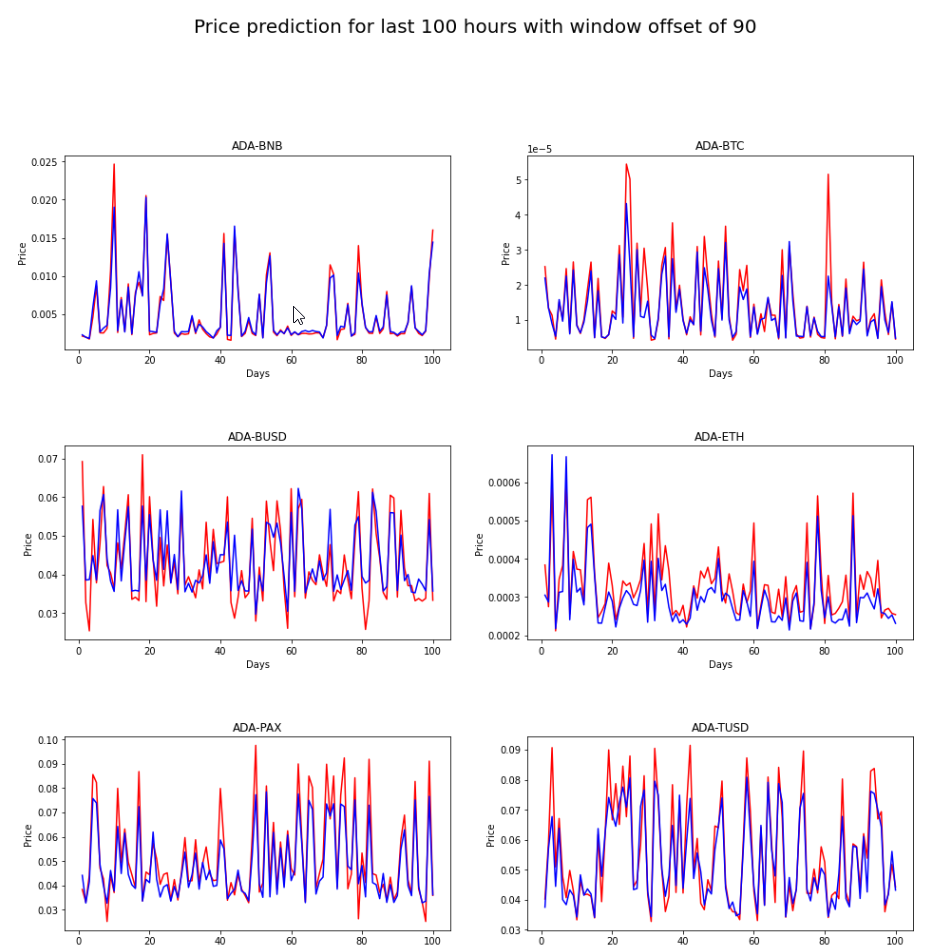
\includegraphics[width=\linewidth]{fig/MLCryptoChart.png}
    \caption{Different predictions after the model has been trained}
    \label{fig:MLCryptoChart}
\end{figure}

\subsection{Newsfeed data set training and tuning}

Trying to tune and adjust the newsfeed data set was even more complicated. The KNN algorithm was used under the premise that as the number of clusters grow for the model to be trained, more differences can be spotted after text processing. The distances between the clusters should increase and get to a state enough to assert and properly distinguish the topics for the articles. On the other hand, a normal sentiment analysis from previously trained models were made just to visualize how much the algorithms could predict the positive or negative impact on specific articles. It was however not possible to segregate the clusters to a distance considerable enough to define topics on the news. This is a limitation addressed in the next section.

\begin{figure}[H]
   \centering
   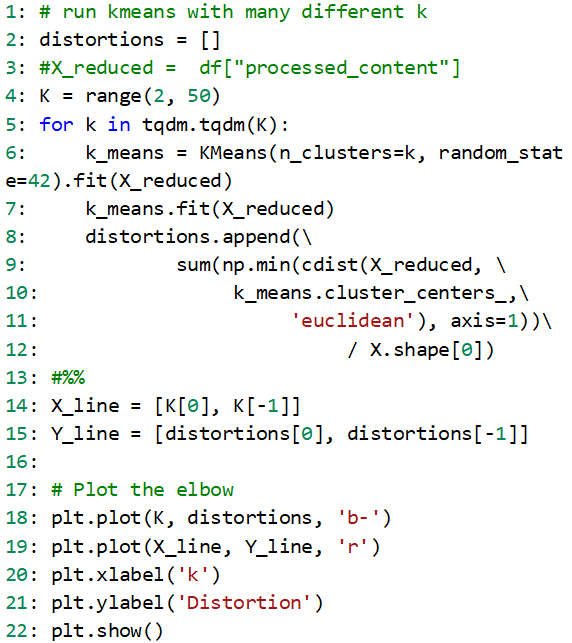
\includegraphics[width=\linewidth]{fig/TextAnalysisDistorions.png}
    \caption{Code snippet to determine the best number of clusters}
    \label{fig:TextAnalysisDistorions}
\end{figure}

\begin{figure}[H]
   \centering
   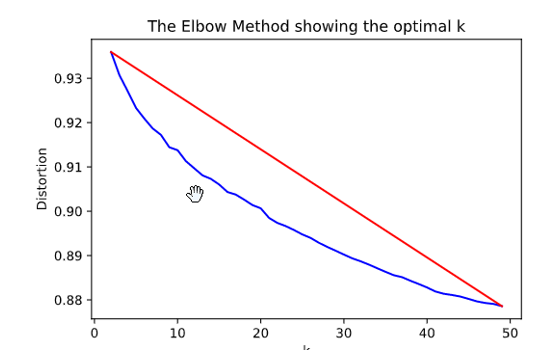
\includegraphics[width=\linewidth]{fig/DistorionChart.png}
    \caption{Results plot to determine proper number of clusters}
    \label{fig:DistorionChart}
\end{figure}


After executing the code from \ref{fig:DistorionChart}, the results to determine a suitable distance between clusters was performed. It was not possible to find a proper distinction between the news, the best fit for KNN cluster classification was 2, which is not suitable for the problem to solve. As the number of clusters increase, it is evident the classification algorithm is not able to distribute properly information among different groups, and therefore different approaches must be performed.



\section{Limitations}
\label{sec:method}
Several limitations were encountered during the project. In some cases, the limitations could be partially avoided by modifying our use case, but in other cases intended implementations had to be dropped and noted as possible future work.

\subsection{Environment resources}

One issue was regarding storage space. The three Virtual machines configured as slave nodes, which would be the machines to hold the data, each had 40 GB of storage. In addition to needing some storage for the operating system and applications needed to run the cluster, the Hadoop Distributed File System (HDFS) would store data across all nodes with redundancy, giving us a limited amount of storage. The Binance data set consisted of 9.36 GB of data in parquet files, and in order to convert this data into a plain text format for use in Machine Learning, it would require up to 72GB on each data node.

This limitation was addressed by performing a parquet file decompression mechanism from Spark, work with the model in memory and saving the trained model once the process was finished. This was a resource intensive mechanism and took more than 6 days to train the whole data set.

\subsection{Data set availability }

No cryptocurrency-related newsfeed data set could be found for use in Machine Learning. Normally to process NLP corpora and perform sentiment analysis over text is now available through different libraries, however it was observed that no pre-trained model nor available data set open to the public has been yet generated. The solution was to create Python scripts for collecting news data (explained in a previous section) and try to exploit the obtained data to obtain relevant results that allowed our data set to be classified. Because the data was unlabeled, using it to train a Machine Learning model would require much more analysis and processing in order to classify the data. Accurate results would require to manually read and label more than 50\% of the news catalog (an equivalent of 15,000 different news) and afterwards used them to train a model and test it over the unlabeled data. This task was so much time consuming and neither of the NLP tools employed to explore the data set provided relevant information that allowed the process to be automated or slightly simplified.

\subsection{Spark state of the art}

The last big limitation encountered, was regarding the execution of Deep Learning algorithms in a distributed fashion. Although already existent SparkML for distributed Machine Learning training on clusters, there is no currently an algorithm available for deep learning process, something necessary required for the provided dataset. Fr this reason TensorFlow must be configured in the cluster to work with Spark, which also created a challenge with regards to distributing the resources when training Machine Learning models. Nevertheless, before implementing Tensorflow natively in python in the cluster an exhaustive research was made to try to address such limitation. It turns out there are already attempts to make deep learning-TensorFlow algorithms to work in a distributed manner under Spark clusters, SparkFlow\cite{lifeomicsparkflow_2020} is a library that tries to implement deep learning on Spark, however, after several attempts to make it work and configure with the TensorFlow algorithms used for the project, several incompatibility issued arose. The final solution therefore was to keep the non-distributed pySpark-TensorFlow approach.


\section{Future Work}
\label{sec:method}
Possible future work includes classifying the collected news data, addressing the limitation discussed in section 8.2. This would allow the training of a Machine Learning model able to perform sentiment analysis on extracted news, labeling data as positive or negative with regards to cryptocurrency market impact.

Combining historical price data and labeled news data, a more accurate model for predicting cryptocurrency prices could be realized. Implementing automatic collection of price and news data on the Hadoop cluster, with the help of real-time sentiment analysis, would allow for a continuously improving prediction model.

Possible further improvements could be made by also considering factors such as technological improvements and social adoption.


\section{Conclusions}
\label{sec:method}
The idea of combining social media information with cryptocurrency trading remains unexplored for the lack of information available. This presents a potential to mature the project as a product with models to be trained on daily basis once new data is released. Although social media keeps nowadays a very important role for cryptocurrency trading decisions, there is no open source dataset nor code available to explore. The code developed for this project is now available on GitHub [8] and Kaggle [7]. It is therefore led for future work to exploit the findings on this project and tune the newsfeed dataset to properly classify it. Social media data such as Twitter would be interesting to be added to find the correlations and perform a Sentiment analysis for the trading decisions on daily basis. There would be, however, an inherent need to previously analyze such dataset. It is important to mention that beforehand the intention was to use any other social media dataset, no results were found, therefore the need to create one by itself. Also the state of the art for distributed systems is not mature enough to address this kind of problems since deep learning cannot be run on clusters yet for parallel computations and calculations, will be very interesting to retake the project and explore future functionalities once this features are released in future versions.

\bibliographystyle{ACM-Reference-Format}
\bibliography{bib/bibliography}
\end{document}
